% To je predloga za poročila o domačih nalogah pri predmetih, katerih
% nosilec je Blaž Zupan. Seveda lahko tudi dodaš kakšen nov, zanimiv
% in uporaben element, ki ga v tej predlogi (še) ni. Več o LaTeX-u izveš na
% spletu, na primer na http://tobi.oetiker.ch/lshort/lshort.pdf.
%
% To predlogo lahko spremeniš v PDF dokument s pomočjo programa
% pdflatex, ki je del standardne instalacije LaTeX programov.

\documentclass[a4paper,11pt]{article}
\usepackage{a4wide}
\usepackage{fullpage}
\usepackage[utf8x]{inputenc}
\usepackage[slovene]{babel}
\selectlanguage{slovene}
\usepackage[toc,page]{appendix}
\usepackage[pdftex]{graphicx} % za slike
\usepackage{setspace}
\usepackage{color}
\definecolor{light-gray}{gray}{0.95}
\usepackage{listings} % za vključevanje kode
\usepackage{hyperref}
\usepackage{float}
\renewcommand{\baselinestretch}{1.2} % za boljšo berljivost večji razmak
\renewcommand{\appendixpagename}{Priloge}

\lstset{ % nastavitve za izpis kode, sem lahko tudi kaj dodaš/spremeniš
language=Python,
basicstyle=\footnotesize,
basicstyle=\ttfamily\footnotesize\setstretch{1},
backgroundcolor=\color{light-gray},
}

\title{Prva domača naloga}
\author{Anže Pečar (63060257)}
\date{\today}

\begin{document}

\maketitle

\section{Uvod}

Cilj prve domače naloge je bil seznaniti se s podatki, ki jih uporablja tekmovanje \textit{JRS 2012 Data Mining Competition: Topical Classification of Biomedical Research Papers}. Podatke smo preučili tako, da smo prešteli primere in atribute, preverili kako redka je matrika in porazdelitve atributov prikazali na različne načine.

\section{Rezultati}

\subsection*{Koliko primerov in atributov vsebujejo podatki?}
Podatki vsebujejo 2000 primerov in 10000 atributov.

\subsection*{Kakšnega tipa so atributi?}
Atributi so zvezni, saj zasedajo vrednosti na intervalu pozitivnih celih števil. 

\subsection*{Kako redka je matrika oz. kakšen delež njenih elementov ima vrednost različen od 0?}
Matrika je precej redka, saj ima le 0.41\% elementov vrednost različno od nič.  

\subsection*{Koliko atributov ima vrednost različno od 0 za posamezen primer?}
\begin{figure}[H]
\begin{center}
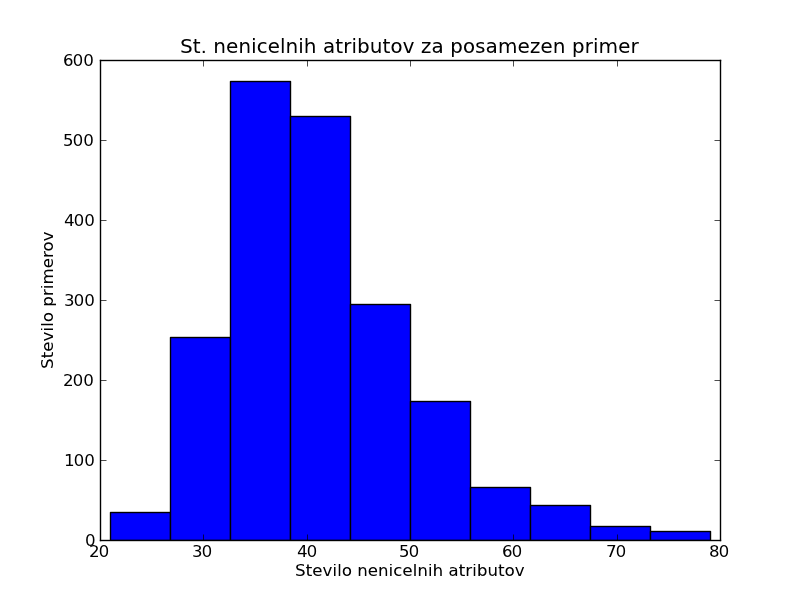
\includegraphics[scale=0.5]{examples.png}
\caption{Prikaz atributov, ki imajo vrednost različno od 0 za posamezen primer}
\label{primeri}
\end{center}
\end{figure}
Iz Slike \ref{primeri}  je lepo razvidno, da ima največ primerov okoli 40 neničelnih atributov. Redki so primeri, ki imajo več kot 70 oz. manj kot 30 atributov.

\subsection*{V koliko primerih atribut zavzame neničelne vrednosti?}
\begin{figure}[H]
\begin{center}
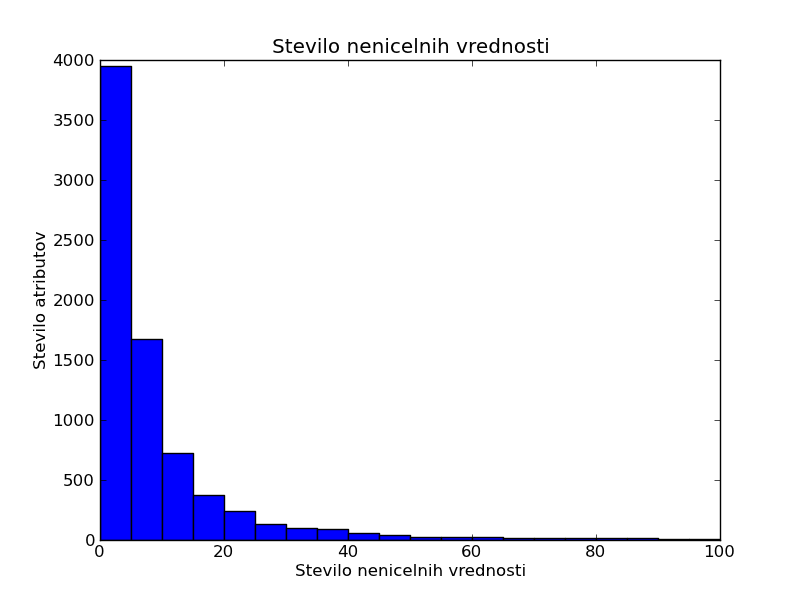
\includegraphics[scale=0.5]{attributes.png}
\caption{Primeri, kjer atribut zavzame neničelne vrednosti}
\label{atributi}
\end{center}
\end{figure}
Iz Slike \ref{atributi} je razvidno, da so zelo redki atributi, ki se pojavijo v več kot 20 primerih. Graf sem omejil na intervalu od 0 do 100, saj ga ostale ničelne vrednosti naredijo manj preglednega.

\subsection*{Koliko je vseh različnih oznak (razredov) v podatkih?}
Vseh različnih oznak v podatkih je 82.

\subsection*{S koliko različnimi oznakami so označeni primeri?}
\begin{figure}[H]
\begin{center}
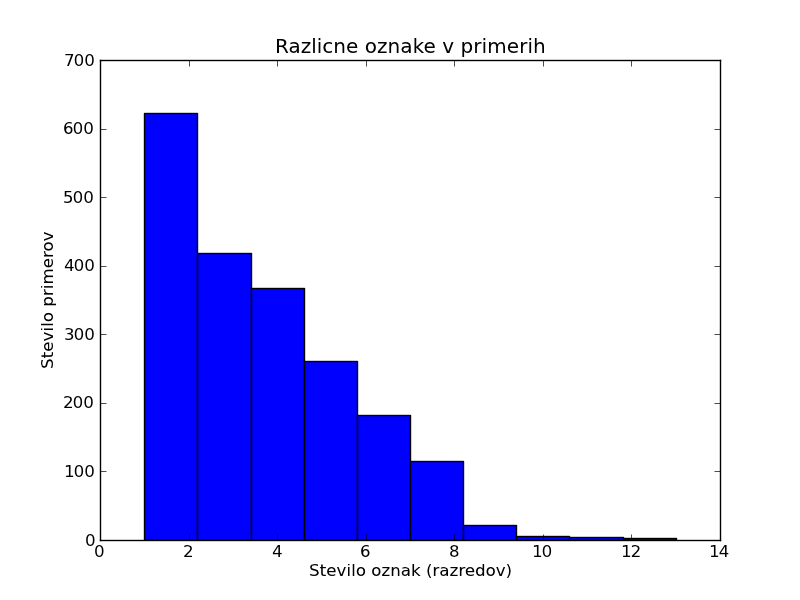
\includegraphics[scale=0.5]{labels.png}
\caption{Različne oznake za primere}
\label{oznake}
\end{center}
\end{figure}
Na Sliki \ref{oznake} lahko vidimo, da ima največ primerov po en razred oz. oznako. Primeri z več kot desetimi oznakami so redki.

\subsection*{Lastno vprašanje 1: Koliko atributov se ne pojavi v nobenem primeru?}
Vprašanje je zanimivo, saj atribute, ki se ne pojavijo v nobenem primeru, lahko odstranimo in poenostavimo nabor podatkov. V našem primeru imamo imamo kar 2349 atributov, ki imajo pri vseh primerih vrednost 0.

\subsection*{Lastno vprašanje 2: Kateri atribut se največkrat pojavi v primerih? V kolikih primerih se pojavi?}
V primerih se največkrat pojavi atribut 7877, ki se pojavi 537 krat.

\subsection*{Lastno vprašanje 3: Naštej 3 najbolj pogoste oznake? Kolikokrat se pojavijo?}
Najpogostejše oznake so:
\begin{itemize}
\item '40' s 502,
\item '44' s 494 in
\item '18' s 428 ponovitvami.
\end{itemize}

\section{Izjava o izdelavi domače naloge}
Domačo nalogo in pripadajoče programe sem izdelal sam.
\end{document}
